\section{Skupinové volání pomocí WebRTC}\label{connectionModels}

Jak bylo zmíněno v části \ref{webRTC}, protokol WebRTC funguje na P2P bázi
\cite{WebRTCORG-PeerConnections}, což přináší otázku, jak využít tuto
technologii pro skupinové volání, kdy je peer klientů potenciálně více než
dva. K řešení tohoto problému existuje několik přístupů, které si následně
rozebereme.

\subsection{Full-mesh}

\begin{figure}[h]
	\centering
	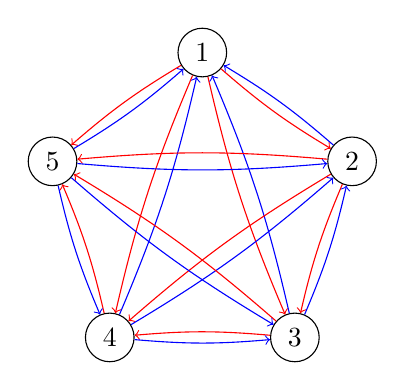
\begin{tikzpicture}[every node/.style={draw,circle}]
		\foreach \i in {1,...,5} {
				\node (\i) at ({(90-360/5*(\i-1))}:2) {\i};
			}
		\foreach \i in {1,...,4} {
				\foreach \j in {\the\numexpr\i+1,...,5} {
						\draw[red,->] (\i) edge[bend right=5] (\j);
						\draw[blue,->] (\j) edge[bend right=5] (\i);
					}
			}
	\end{tikzpicture}
	\caption{Full-mesh}
	\label{fullMeshFig}
\end{figure}

Prvním způsobem je tzv. spojení \textit{full-mesh}, v rámci kterého každý klient
komunikuje s každým dalším klientem, jak je zobrazeno na obrázku
\ref{fullMeshFig}. Hlavní výhodou tohoto přístupu je, že nevyžaduje žádné
\textit{backend komponenty} (servery) -- není tedy třeba vývojářů, kteří by na
backendu pracovali, a zároveň není nutné vkládat finanční prostředky do jeho
provozu. Nehrozí ani, že při selhání backendu by se uživatelé klientů nemohli
spojit. Tento přístup má ale bohužel také mnoho nevýhod
\cite{HalOpenScience-SFUs}.

První může být složitější vytvoření samotného spojení dvou klientů --
v~klasickém P2P modelu obvykle dochází k tomu, že jeden uživatel volá druhého,
to samé ale u full-mesh spojení platit nemusí. Když se nový uživatel pokouší
připojit do skupinového hovoru, je nejasné, zda jeho klient volá klienty, kteří
se hovoru již účastní, či naopak. Je sice možné definovat příslušné pravidlo,
ale v případě, že se dva uživatelé pokusí připojit ve stejný okamžik, je situace
komplikovanější, neboť nelze jednoznačně určit, kdo je volající a~kdo volaný.
Jedním řešením jsou tzv. \textit{algoritmy pro glare resolution}, které řeší
situaci, kdy se klienti snaží kontaktovat navzájem ve stejný okamžik. Obvykle
každý klient vygeneruje náhodné číslo, které je poté v případě, že dochází ke
\textit{glare} situaci, porovnáno s číslem druhého klienta a klient s větším či
menším číslem (záleží na implementaci) je pak vybrán jako volající
\cite{MagnusWesterlund-GlareInWebRTC}. Někdy také dochází k lexikografickému
porovnání identifikátorů klientů pro zvolení klienta, který bude kontaktovat
toho druhého \cite{GitHub-MSC3401}.

Full-mesh spojení má také nevýhodu v tom ohledu, že může častěji docházet k tzv.
\textit{split-brains} \cite{StephenHaddock-SplitBrainAvoidance}. Protože je
každý klient spojen s každým dalším klientem, je spojení velmi náchylné k
chybám, hrozí tedy, že jeden z klientů budu přijímat streamy jen od určité
podskupiny klientů, zatímco jiný klient bude přijímat stream od jiné podskupiny
klientů, a tak dva uživatelé, kteří se hovoru účastní, můžou mít značně odlišný
zážitek.

Dalším problémem je zátěž klienta, protože musí přijímat RTP streamy všech
klientů, které nejdříve rozšifrovává a dekóduje. Zároveň posílá všechny své RTP
streamy ostatním klientům, ty musí naopak enkódovat a následně zašifrovat. Při
vyšším počtu klientů v hovoru je pak třeba, aby všichni klienti běželi na
dostatečně silném hardwaru
\cite{BBC-FirstWebcamMadeCoffeePotFamous,Red5Pro-WebRTCScalingApproaches}.

Další bariérou je internetové přípojení -- většina klientů totiž nemá dostatečně
rychlou síť, aby mohli posílat RTP streamy všem uživatelům, a tak je realisticky
možné pomocí full-mesh spojení provádět jen hovory v nižších počtech klientů
(obvykle je maximum 5 - 8 klientů) \cite{BlogGeek-WebRTCP2PMesh}.

\subsection{Servery -- foci}

Možným řešením problémů s full-mesh spojením je využití backendu. V~tomto
případě bude každý klient posílat své RTP streamy serveru, ze kterého se tedy
stává tzv. \textit{focus} (bod, ve kterém jsou jednotlivé streamy soustředěny;
množné číslo je \textit{foci}). Tento focus poté streamy přeposílá ostatním
klientům. Existují zde dva hlavní přístupy
\cite{Red5Pro-WebRTCScalingApproaches}, které si níže rozebereme.

\subsubsection{Multipoint Control Unit}

\begin{figure}[h]
	\centering
	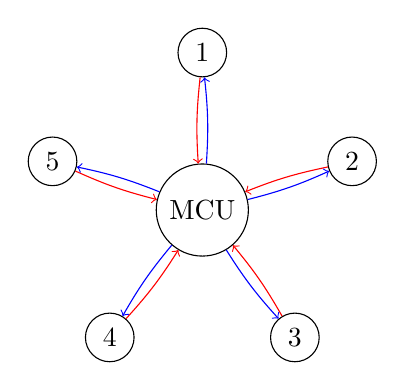
\begin{tikzpicture}[every node/.style={draw,circle}]
		\node (MCU) at (0,0) {MCU};

		\foreach \i in {1,...,5} {
				\node (\i) at ({90-360/5*(\i-1)}:2) {\i};
			}
		\foreach \i in {1,...,5} {
				\draw[red,->] (\i) edge[bend right=5] (MCU);
				\draw[blue,->] (MCU) edge[bend right=5] (\i);
			}
	\end{tikzpicture}
	\caption{Multipoint Control Unit}
	\label{mcu}
\end{figure}

První možností je tzv. \textit{Multipoint Control Unit} (dále \textit{MCU}),
tento server přijímá streamy jednotlivých klientů a následně je transkóduje a
mixuje do jednoho, který pak zpět posílá všem uživatelům (viz obrázek č.
\ref{mcu}). Hlavní výhodou tohoto přístupu je, že klient nemusí mít vysoký ani
download, neboť přijímá jen jeden stream. Má ale relativně dost nevýhod
\cite{Red5Pro-WebRTCScalingApproaches}.

První z nich je, že streamy jsou mixované do jednoho streamu, který je pak pro
všechny klienty stejný, neumožňuje tedy uživatelům klientů, aby si vybrali,
který stream budou sledovat atp.
\cite{Red5Pro-WebRTCScalingApproaches}.

Zároveň proces transkódování a mixování je poměrně náročný na výkon, příslušný
server tedy potřebuje silný hardware. Tento proces je také mírně časově náročný,
což znamená, že uživatelé vidí a slyší věci s mírným
zpožděním~\cite{Red5Pro-WebRTCScalingApproaches}.

Poslední nevýhodou, kterou zmíníme, je to, že aby server mohl streamy
transkódovat a mixovat, je nutné, aby je nejdříve rozšifroval, což znamená, že z
principu není možné, aby komunikace mezi klienty byla
E2EE~\cite{ITSecurityKnowHow-E2EGainsANewMeaning}.

\subsubsection{Selective Forwarding Unit}

\begin{figure}[h]
	\centering
	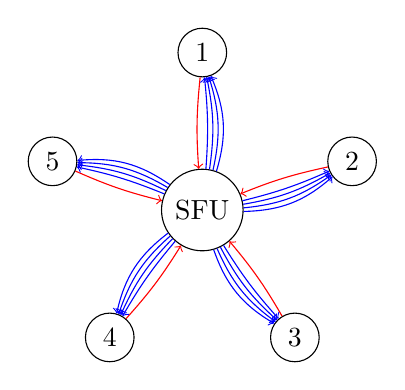
\begin{tikzpicture}[every node/.style={draw,circle}]
		\node (SFU) at (0,0) {SFU};

		\foreach \i in {1,...,5} {
				\node (\i) at ({90-360/5*(\i-1)}:2) {\i};
			}
		\foreach \i in {1,...,5} {
				\draw[red,->] (\i) edge[bend right=5] (SFU);
				\foreach \j in {1,...,4} {
						\draw[blue,->] (SFU) edge[bend right=5*\j] (\i);
					}
			}
	\end{tikzpicture}
	\caption{Selective Control Unit}
	\label{sfu}
\end{figure}

Druhou možností je tzv. \textit{Selective Forwarding Unit} (dále \textit{SFU}),
tento server přijímá streamy jednotlivých klientů a následně podskupinu těchto
streamů přeposílá ostatním klientům \cite{HalOpenScience-SFUs}, jak je vidět na
obrázku č. \ref{sfu}.

Toto řešení má několik výhod -- umožňuje E2EE, neboť nepotřebuje streamy
transkódovat a mixovat \cite{WebRTCHacks-TrueE2EE}. Z tohoto důvodu také nemá
takové požadavky na hardware, jednotlivé streamy jsou klientům posílány
samostatně, takže si uživatel může zvolit, co bude sledovat
\cite{Red5Pro-WebRTCScalingApproaches}. Zároveň tento model umožňuje tzv.
\textit{federaci} (více v částech \ref{matrix} a \ref{matrixRTC}).

\begin{figure}[h]
	\centering
	\begin{tikzpicture}[every node/.style={rectangle, rounded corners=2mm}]
		\foreach \i in {1,...,3} {
				\node[draw,minimum size=24mm] (\i) at (-5, 6-3*\i) {\i};
			}

		\node[draw,minimum height=9cm] (SFU) at (0,0) {SFU};

		\foreach \i in {4,...,5} {
				\node[draw,minimum size=24mm] (\i) at (5, 13.5-3*\i) {\i};
			}

		\foreach \i in {1,...,3}{
				\foreach \j in {0,...,2} {
						\FPeval{\result}{round(720/(2^(\j)):0)}

						\draw[red,->] ([yshift=(0.75*\j-0.75)*1cm]\i.east) -- ([yshift=(((6-3*\i)-(1-\j*1))*1cm)]SFU.west) node[midway, anchor=south]
						{{\result}p};
					}
			}

		\draw[blue,->] ([yshift=1.5cm]SFU.east) -- (4.west) node[midway, anchor=south] {720p};
		\foreach \j in {1,...,3} {
				\draw[blue,->] ([yshift=(0.5-\j)*1cm]SFU.east) -- ([yshift=(1.5-0.75*\j)*1cm]5.west) node[midway, anchor=south] {180p};
			}
	\end{tikzpicture}
	\caption{Simulcast}
	\label{simulcast}
\end{figure}

Oproti MCU sice vyžaduje větší download ze strany klientů, neboť přijímají
streamy jednotlivě. Toto ale není tak velký problém, neboť SFU může posílat jen
určitou podskupinu streamů. Zároveň existuje metoda s názvem \textit{simulcast},
kdy klient SFU posílá několik verzí svých streamů v různých rozlišeních (obvykle
jsou to původní, poloviční a čtvrteční) a s různým počtem snímku za sekundu, SFU
poté přeposílá vhodnou verzi streamu (viz \ref{simulcast}). Vhodná verze se
obvykle vybírá na základě několika kritérií. Prvním z~nich často je, v jakém
rozlišení bude video zobrazeno na koncovém klientovi -- např. jestli má uživatel
jedno video velkém rozlišení a ostatní jsou malá, nebo či má všechny videa
zobrazena ve stejném rozlišení bez toho, aby nějaké bylo zvětšené. Dalším
faktorem při výběru je spojení s jednotlivým klienty a jeho kvalita
\cite{LiveKit-SimulcastIntroduction}.
